

\begin{table}[h]
\begin{tabular}{c|c|c|c|c|}
\cline{2-5}
\textbf{} &
  \multicolumn{2}{p{5cm}|}{\textbf{Only use data collected by current agent}} &
  \multicolumn{2}{c|}{\textbf{Use data collected by other agents}} \\ \hline
\multicolumn{1}{|p{3cm}|}{\textbf{Data collection using current agent}} &

  \multicolumn{2}{c|}{\begin{tabular}[c]{@{}c@{}}
  
Online, on-policy RL 

%   \raisebox{-\totalheight}{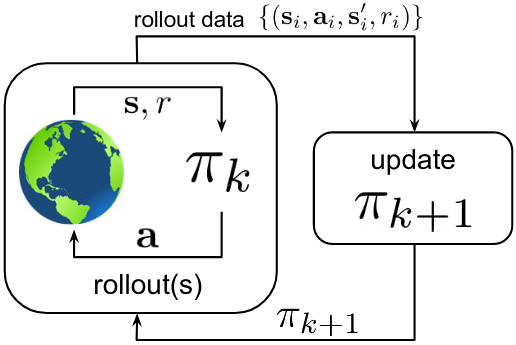
\includegraphics[width=5cm]{figures/on-policy.png}}
%   \vspace{5mm} 
  
  \end{tabular}} &
  
  \multicolumn{2}{c|}{\begin{tabular}[c]{@{}c@{}}
  
Online, off-policy RL 

%   \raisebox{-\totalheight}{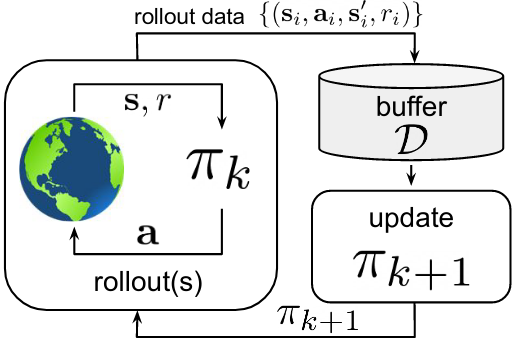
\includegraphics[width=5cm]{figures/off-policy.png}}
%   \vspace{5mm} 
  
  \end{tabular}} \\ \hline
  
\multicolumn{1}{|p{3cm}|}{\textbf{Fixed dataset (no additional data collection)}} &
  \multicolumn{2}{c|}
  {-} 
  &
  \multicolumn{2}{c|}{\begin{tabular}[c]{@{}c@{}}
  
  Offline (fully off-policy) RL 
  
%   \raisebox{-\totalheight}{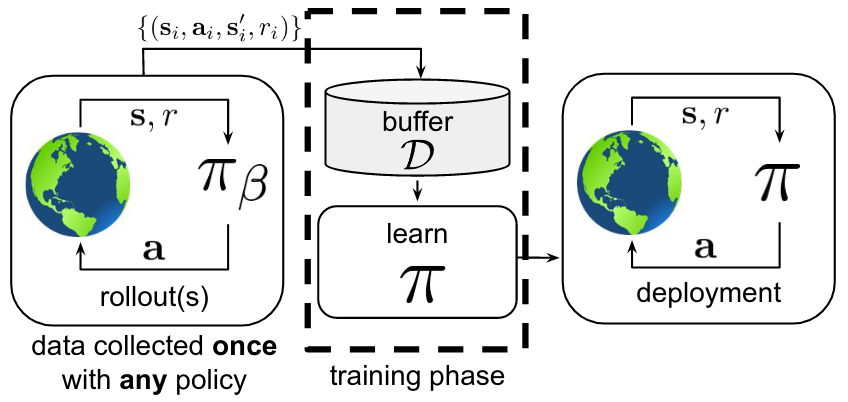
\includegraphics[width=7cm]{figures/offline.png}}
  
  \end{tabular}} \\ \hline
\end{tabular}
\caption{Classification of RL algorithms \cite{Google_offline_RL}.}
\label{tab:RL-classification}
\end{table}
